\section{Motion of a Mass Connected to a Spring}
\label{sec:motion_of_a_mass_connected_to_a_spring}	

\subsection*{Recommended Tutorials:}
\begin{itemize}[noitemsep]
	\item \nameref{chp:differential_equations}, pg. \pageref{chp:differential_equations}
	    \index{differential equations!}
\end{itemize}

\subsection*{Introduction:}
\begin{marginfigure}
    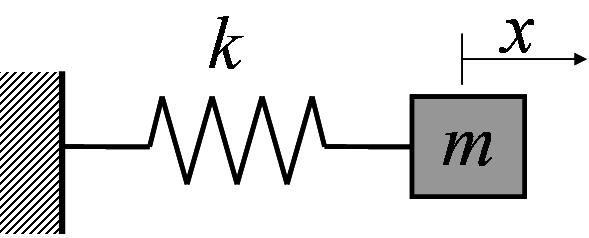
\includegraphics[scale=0.5]{activities/math122/figures/mass_spring.png}
    \caption{A mass on a spring, where $k$ is the spring constant and $x$ measures the displacement of the mass from the equilibrium position ($x=0$).}
    \label{fig:mass_spring}
\end{marginfigure}
According to Hooke's law ($F=-kx$) and Newton's second law ($F=ma$), the differential equation for the motion of a mass ($m$) on the end of a spring is 
\begin{equation*}
m \frac{d^2x}{dt^2}=-kx,
\end{equation*}
    \index{differential equations!hooke's law}
where $k$ is the spring constant (a measure of the stiffness of the spring). This equation assumes no damping (resistance). The displacement of the mass from equilibrium is denoted by $x$, and thus $\frac{dx}{dt}$ is the velocity, and $\frac{d^2x}{dt^2}$ is the acceleration. 

If we add damping (resistance) to the spring, then the damping is opposite the direction of the motion and proportional to the velocity. Therefore we have the equation,
\[ m \frac{d^2x}{dt^2}=-kx-c\frac{dx}{dt}, \]
where $c$ is the damping constant. 

For the exercises, we will assume that the mass is $m=2$-kg and the spring constant is $k=3$ kg/s$^2$. We will look at the equation of motion with no damping ($c=0$), overdamping ($c=4$ kg/s), and underdamping ($c=0.5$ kg/s).

In all cases, we will use the initial conditions $x(0)=1$ m and $x'(0)=-1$ m/s.

\subsection*{Exercises:}

\begin{enumerate}
\item Consider the equation of motion of a $2$-kg mass attached to a spring with $k=3$ kg/s$^2$.
\label{ex:mass_spring_nodamping}
\[ 2 x''(t) = -3 x(t). \]
\begin{enumerate}
    \item Solve the differential equation using the given initial conditions.
    \item Plot the solution of the differential equation.
    \marginnote{The \texttt{rhs()} command may be used to refer to only the right hand side of the differential equation solution. You can use this command to assign a name to the solution.}
    \item Insert a new paragraph and describe what you observe about the motion of a mass on the spring.
        \index{differential equations!rhs()}
\end{enumerate}
\clearpage



\item Consider the equation of motion of a $2$-kg mass attached to a spring with $k=3$ kg/s$^2$ and a damping constant of $c=4$ kg/s. This is considered \textbf{overdamping}.
\[2 x''(t) = -3 x(t) - 4 x'(t).\] \marginnote[-2.5cm]{The solutions to these differential equations will be sine and cosine functions of the form \[\sin(kt) \text{ and } \cos(kt).\] The period $T$ of these oscillations may be found using the formula \[T=\frac{2\pi}{k}.\] }
    \index{mathematical functions!sine}
     \index{mathematical functions!cosine}
     \vspace{-.8cm}
\begin{enumerate}
    \item Solve the differential equation using the given initial conditions.
    \item Plot the solution of the differential equation.
    \item Insert a new paragraph and describe what you observe about the motion of a mass on the spring with overdamping.
\end{enumerate}

\item Consider the equation of motion of a $2$-kg mass attached to a spring with $k=3$ kg/s$^2$ and a damping constant of $c=0.5$~kg/s. This is considered \textbf{underdamping}.
\label{ex:mass_spring_underdamping}
\[ 2 x''(t) = -3 x(t) - 0.5 x'(t). \]
\begin{enumerate}
    \item Solve the differential equation using the given initial conditions.
    \item Plot the solution of the differential equation.
    \item Insert a new paragraph and describe what you observe about the motion of a mass on the spring with underdamping.
\end{enumerate}

\marginnote[-3cm]{To solve these differential equations algebraically you assume that solutions are of the form $x(t)={\rm e}^{rt}$ and then plug it into the differential equation to get the ``characteristic equation" to solve for $r$. If the roots are complex, you will have oscillations (sine and cosine functions) and if the roots are real, then you have strictly exponential solutions. Notice that the overdamped case has no oscillations whereas the underdamping and no-damping cases have oscillations in their solutions.}
     \index{mathematical functions!exponential}

\item Suppose we wish to force the spring to oscillate at a given frequency. Let's add a forcing term $3 \sin(2t)$ to the undamped equation of motion from exercise \ref{ex:mass_spring_nodamping}.
\label{ex:mass_spring_forcing}
\[ 2x''(t) = -3 x(t) + 3\sin(2t) \]
\begin{enumerate}
    \item Solve the differential equation using the given initial conditions.
    \item Plot the differential equation solution.
    \item Insert a new paragraph and describe what you observe about the motion of a mass on the spring with \textbf{forcing and no damping}.
\end{enumerate}

\item Let's add damping to equation of motion from exercise \ref{ex:mass_spring_forcing} with a damping constant of $0.5$ kg/s.
\[ 2x''(t) = -3 x(t) - 0.5 x'(t) + 3\sin(2t) \] 
\begin{enumerate}
    \item Solve the differential equation using the given initial conditions.
    \item Plot the differential equation solution.
    \item Insert a new paragraph and describe what you observe about the motion of a mass on the spring with \textbf{forcing and underdamping}.
\end{enumerate}

\end{enumerate}